\documentclass[hyperref,german,beleg,noproblem,notoc,plainarticle]{cgvpub}

\makeatletter
\def\BState{\State\hskip-\ALG@thistlm}
\makeatother
\DeclareMathOperator*{\argmax}{arg\,max}  % in your preamble
\DeclareMathOperator*{\argmin}{arg\,min}  % in your preamble 


%weitere Optionen zum Erg�nzen (in eckigen Klammern):
%
% female	weibliche Titelbezeichnung bei Diplom
% bibnum	numerische Literaturschl�ssel
% final 	f�r Abgabe	
% lof			Abbildungsverzeichis
% lot			Tabellenverzeichnis
% noproblem	keine Aufgabenstellung
% notoc			kein Inhaltsverzeichnis
% twoside		zweiseitig
\author{\textbf{Gruppe 11}\\ Cao,Bozhi\hspace{1em}Gao,Yue\hspace{1em}Jia,Xuehua\hspace{1em}Zhu,Jinyao }
\title{PRAKTIKUMSAUFGABE II}
%\bibfiles{literatur}
%\problem{Text der Aufgabenstellung...}
%\copyrighterklaerung{Hier soll jeder Autor die von ihm eingeholten
%Zustimmungen der Copyright-Besitzer angeben bzw. die in Web Press
%Rooms angegebenen generellen Konditionen seiner Text- und
%Bild"ubernahmen zitieren.}
%\acknowledgments{Die Danksagung..}

\renewcommand\thesection{\arabic{section}.}
\renewcommand\thesubsection{\thesection\arabic{subsection}}
\renewcommand\thefigure{\arabic{figure}}  


\begin{document}
	  
\section{Aufgabe}
\subsection{Signalflussplan}
siehe Programm: \textbf{A1\_Hydropulszylinder.mdl}
\subsection{Servoventil testen:}
siehe Programm: \textbf{A1\_Servoventil\_Test.mdl}
\subsection{Verifikation:}
siehe Programm: \textbf{a1\_main.m}
\section{Aufgabe}
\subsection{Berechnung der Transitionsmatrix und diskrete Eingangsmatrix:}
siehe Programm: \textbf{a2\_main.m}
\subsection{Vergleichen(mit nichtlineares kontinuierliches Modell):}
siehe Programm: \textbf{a2\_main.m} und \textbf{A2\_compare\_c\_d.mdl}
\section{Aufgabe}
\subsection{Dimensionierung der Reglerverst"arkung:}
siehe Programme: \textbf{a3\_main.m} und \textbf{A3\_control\_loop\_tune.mdl}
\subsection{Geschlossener Regelkreis mit linearem zeit-diskreten Streckenmodell:}
siehe Programm:  \textbf{a3\_main.m} und \textbf{A3\_control\_loop\_lin\_d\_model.mdl}\\
\textbf{Kritische Reglerverst"arkung:} $K_{\mathrm{I,krit}}\approx2.215$.

\section{Aufgabe}
\subsection{Geschlossener Regelkreis mit nichtlinearem kontinuierlichem Streckenmodell:}
siehe Programm: \textbf{a4\_main.m} und \textbf{A4\_control\_loop\_nlin\_c\_model.mdl}
\subsection{Vergleichen mit dem linearen zeit-diskreten Streckenmodell:}
\begin{figure}[htb]
	\centering
	$
	\begin{array}{cc}
	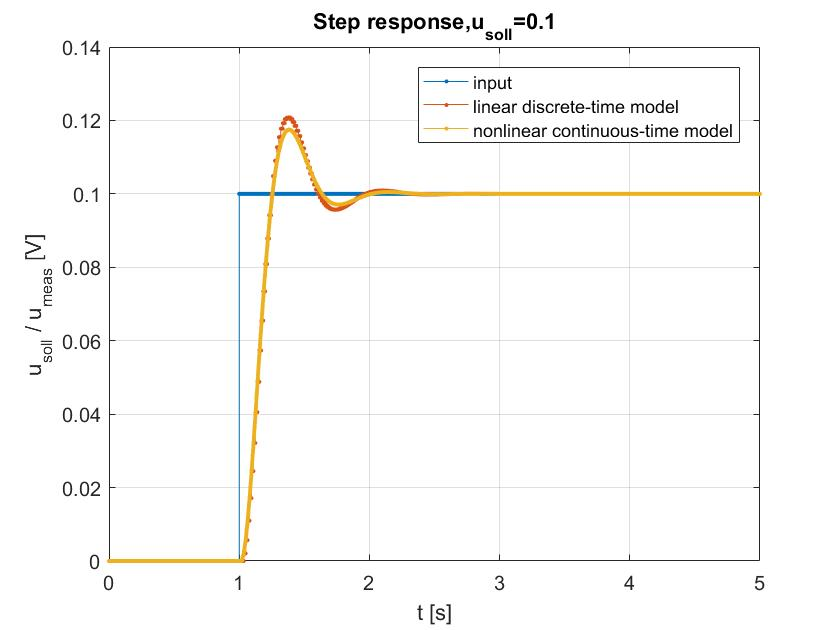
\includegraphics[width=0.45\linewidth]{picture/a4_1} &
	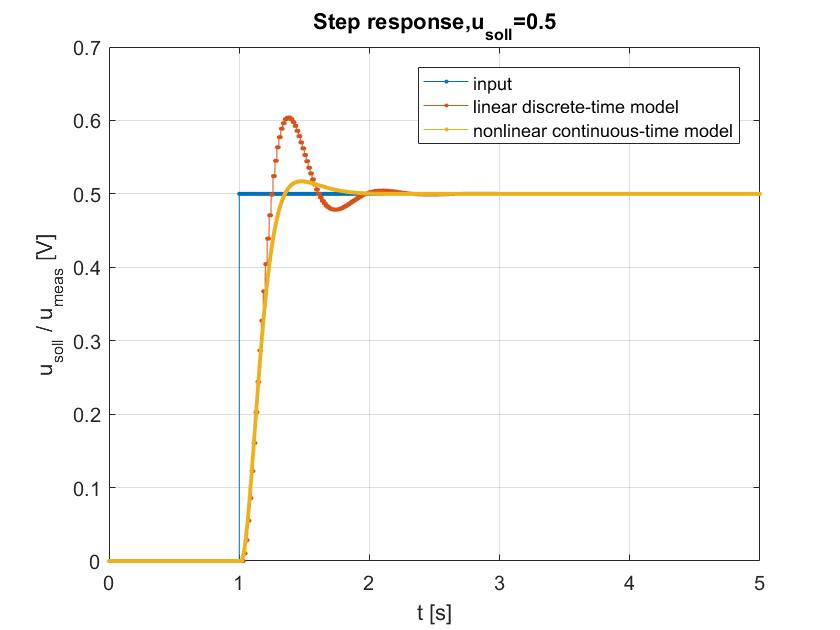
\includegraphics[width=0.45\linewidth]{picture/a4_2}\\
	\text{(a)} &  \text{(b)}\\
	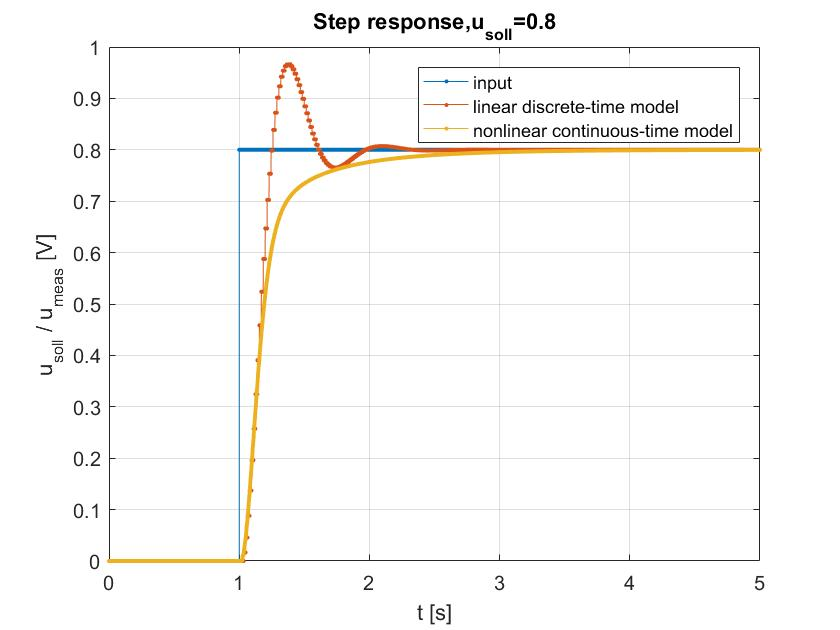
\includegraphics[width=0.45\linewidth]{picture/a4_3} & \\
	\text{(c)} & \\
	\end{array}
	$
	\caption{(a) $u_{\mathrm{soll}}=0.1$; (b) $u_{\mathrm{soll}}=0.5$; (c) $u_{\mathrm{soll}}=0.8$;}
	\label{fig1}
\end{figure}
\textbf{Bemerkung:}\\ je weiter der $u_{\mathrm{soll}}$ von Null entfernt ist, desto gr"o"ser sind die Differenzen(auch Linearisierungsfehler) zwischen dem linearen zeit-diskreten und dem nichtlinearen zeit-kontinuierlichen Modell.
\newpage
\subsection{Kritische Reglerverst"arkungen:}
\begin{table}[htb]
\centering
\begin{tabular}{c||c|c|c}
\hline 
$u_{\mathrm{soll}}$ & 0.1 & 0.5 & 0.8 \\
\hline 
$K_{\mathrm{I,krit}}$ & 2.46 & 4.9 & 15 \\
\hline 

\end{tabular} 
\end{table}
\end{document} 